\documentclass{article}


% 中文支持
\usepackage[UTF8,heading = true]{ctex}


% 页面布局
\usepackage[a4paper]{geometry}
\usepackage{fancyhdr}
\pagestyle{fancy}
\newcommand{\Lhead}[1]{\fancyhead[L]{#1}}
\newcommand{\Chead}[1]{\fancyhead[C]{#1}}
\newcommand{\Rhead}[1]{\fancyhead[R]{#1}}
\newcommand{\Lfoot}[1]{\fancyfoot[L]{#1}}
\newcommand{\Cfoot}[1]{\fancyfoot[C]{#1}}
\newcommand{\Rfoot}[1]{\fancyfoot[R]{#1}}
\renewcommand{\headrulewidth}{0.4pt}
\renewcommand{\footrulewidth}{0pt}
\usepackage{lastpage}
%待填信息
% -----------------------------------------------------
\newcommand{\Course}{深度学习平台与应用}             		%      |
\newcommand{\Assignment}{深度学习作业 2}		  %      | 
\newcommand{\Name}{田永铭}				    	 %      |
\newcommand{\ID}{221900180}				  	   %       |
\newcommand{\Email}{tianym2022@smail.nju.edu.cn}  %    |
% ------------------------------------------------------
\fancyhead[L]{\Course}
\fancyhead[C]{\Assignment}
\fancyhead[R]{\ID \Name}
\fancyfoot[C]{\thepage\ / \pageref*{LastPage}}	
\setlength\headheight{36pt}
% 自定义页面样式第一页只有页脚没有页眉
\makeatletter
\def\ps@onlyfoot{
	\let\@oddhead\@empty
	\let\@evenhead\@empty
	\def\@oddfoot{\hfil\thepage\ / \pageref*{LastPage}\hfil}
	\def\@evenfoot{\hfil\thepage\ / \pageref*{LastPage}\hfil}
}
\makeatother
% maketitle
\title{\Huge\Assignment}
\author{\ID \Name \quad\href{mailto:tianym2022@smail.nju.edu.cn}{\color{magenta}\Email}}
\date{\today}


% 字体和颜色
\usepackage{fontspec} 
\fontsize{12pt}{\baselineskip}\selectfont
\usepackage{xcolor}


% 数学支持
\usepackage{amssymb}
\usepackage{amsfonts}
\usepackage{amsmath}
\usepackage{esint}
\usepackage{gensymb}
\usepackage{mathtools}
\usepackage{amsthm}

% 左边大括号
%\[
%\left\{
%\begin{aligned}
%	& \text{approximate  covariance matrix of GP} \\
%	& \text{only use subset}\\
%	& \text{conditional independence assumption}
%\end{aligned}
%\right.
%\]

% 矩阵
%\[
%\begin{matrix}
%	a & b \\
%	c & d
%\end{matrix}
%\]

% 行列式
%\[
%\begin{vmatrix}
%	a & b \\
%	c & d
%\end{vmatrix}
%\]


% 标题格式
\usepackage{titlesec}
% 自定义 section 标题格式
\renewcommand{\thesection}{\chinese{section}、}
\titleformat{\section}
{\normalfont\Large\bfseries\centering\color[rgb]{0,0,0.8}} % 设定字体和大小
{\thesection}{0em} % 设定编号和标题之间的距离
{}
% 自定义 subsection 标题格式
\renewcommand{\thesubsection}{\arabic{section}.\arabic{subsection} }
\titleformat{\subsection}
{\normalfont\large\bfseries\color[rgb]{0.23,0.65,0.99}}
{\thesubsection}{0em}
{}
% 自定义 subsubsection 标题格式
\renewcommand{\thesubsubsection}{\arabic{section}.\arabic{subsection}.\arabic{subsubsection} }
\titleformat{\subsubsection}
{\normalfont\normalsize\bfseries}
{\thesubsubsection}{0em}
{}
% 设置 section 标题的间距
\titlespacing*{\section}
{0pt}{3.5ex plus 1ex minus .2ex}{2.3ex plus .2ex}
% 设置 subsection 标题的间距
\titlespacing*{\subsection}
{0pt}{3.25ex plus 1ex minus .2ex}{1.5ex plus .2ex}
% 设置 subsubsection 标题的间距
\titlespacing*{\subsubsection}
{0pt}{3.25ex plus 1ex minus .2ex}{1.5ex plus .2ex}


% 代码 
% 如非默认，需使用[language=xxx,style=mystyle]
\usepackage{listings}
% language:  {[x86masm]Assembler}(汇编); python; C; C++; Java; SQL; Matlab; R; bash; make(makefile)
\lstdefinestyle{mystyle}{
	basicstyle=\ttfamily\small,
	numbers=left,
	numberstyle=\tiny\color{magenta},
	stepnumber=1,
	numbersep=10pt,
	backgroundcolor=\color[rgb]{0.95,0.95,0.95},
	showspaces=false,
	showstringspaces=false,
	showtabs=false,
	frame=single,
	rulecolor=\color{black},
	tabsize=2,
	captionpos=b,
	breaklines=true,
	breakatwhitespace=false,
	title=\lstname,
	keywordstyle=\color{blue},
	commentstyle=\color[rgb]{0.0,0.5,0.0},
	stringstyle=\color[rgb]{0.23,0.65,0.99}\itshape,
	escapeinside={\%*}{*)},
	morekeywords={}, % 添加更多关键字
	literate=
	{[}{{{\color{red}[}}}1
	{]}{{{\color{red}]}}}1
	{\{}{{{\color[rgb]{0.9,0,0.9}\{}}}1
	{\}}{{{\color[rgb]{0.9,0,0.9}\}}}}1
%	{0}{{{\color[rgb]{0.2,0.9,0.4}0}}}1
%	{1}{{{\color[rgb]{0.2,0.9,0.4}1}}}1
%	{2}{{{\color[rgb]{0.2,0.9,0.4}2}}}1
%	{3}{{{\color[rgb]{0.2,0.9,0.4}3}}}1
%	{4}{{{\color[rgb]{0.2,0.9,0.4}4}}}1
%	{5}{{{\color[rgb]{0.2,0.9,0.4}5}}}1
%	{6}{{{\color[rgb]{0.2,0.9,0.4}6}}}1
%	{7}{{{\color[rgb]{0.2,0.9,0.4}7}}}1
%	{8}{{{\color[rgb]{0.2,0.9,0.4}8}}}1
%	{9}{{{\color[rgb]{0.2,0.9,0.4}9}}}1
}
\lstset{style=mystyle}


% 图表
\usepackage{graphicx}
\usepackage{booktabs}
\usepackage{caption}
\captionsetup{font={small}}
\usepackage{diagbox}
\usepackage{array}
\usepackage{pgfplots}
\pgfplotsset{compat=1.17}

% 表1
%\begin{table}[h!]
%	\centering
%	\caption{Performance comparison on mini-ImageNet and tiered-ImageNet datasets.}
%	\begin{tabular}{@{}lcccccccc@{}}
%		\toprule
%		Dataset & Method & Backbone & 5-way 1-shot \\
%		\midrule
%		\multirow{9}{*}{\rotatebox[origin=c]{90}{mini-ImageNet}} 
%		& ProtoNet & Conv-4 & 46.291 \\
%		& MAML & Conv-4 & 49.704 \\
%		& BOIL & Conv-4 & 48.456 \\
%		& CAN & ResNet-12 & 59.493\\
%		& LEO & ResNet-12 & 55.056 \\
%		& SKD & ResNet-12 & 66.700  \\
%		& R2D2 & ResNet-12 & 59.802 \\
%		& DiffKendall (Ours) & ResNet-12 & \textbf{68.727} \\
%		\midrule
%		\multirow{6}{*}{\rotatebox[origin=c]{90}{tiered-ImageNet}} 
%		& ProtoNet & Conv-4 & 46.653 \\
%		& Relation Networks & Conv-4 & 55.107  \\
%		& MAML & Conv-4 & 51.038 \\
%		& R2D2 & ResNet-12 & 64.916  \\
%		& DiffKendall (Ours) & ResNet-12 & \textbf{66.598} \\
%		\bottomrule
%	\end{tabular}
%\end{table}

% 表2
%\begin{table}[t]
%	\caption{Classification accuracies for naive Bayes and flexible
%		Bayes on various data sets.}
%	\label{sample-table}
%	\vskip 0.15in
%	\begin{center}
%		\begin{small}
%			\begin{sc}
%				\begin{tabular}{lcccr}
%					\toprule
%					Data set & Naive & Flexible & Better? \\
%					\midrule
%					Breast    & 95.9$\pm$ 0.2& 96.7$\pm$ 0.2& $\surd$ \\
%					Cleveland & 83.3$\pm$ 0.6& 80.0$\pm$ 0.6& $\times$\\
%					Glass2    & 61.9$\pm$ 1.4& 83.8$\pm$ 0.7& $\surd$ \\
%					Credit    & 74.8$\pm$ 0.5& 78.3$\pm$ 0.6&         \\
%					Horse     & 73.3$\pm$ 0.9& 69.7$\pm$ 1.0& $\times$\\
%					Meta      & 67.1$\pm$ 0.6& 76.5$\pm$ 0.5& $\surd$ \\
%					Pima      & 75.1$\pm$ 0.6& 73.9$\pm$ 0.5&         \\
%					Vehicle   & 44.9$\pm$ 0.6& 61.5$\pm$ 0.4& $\surd$ \\
%					\bottomrule
%				\end{tabular}
%			\end{sc}
%		\end{small}
%	\end{center}
%	\vskip -0.1in
%\end{table}


% 算法
%\usepackage{algorithm}
%\usepackage{algorithmic}
%\begin{algorithm}[tb]
%	\caption{Bubble Sort}
%	\label{alg:example}
%	\begin{algorithmic}
	%		\STATE {\bfseries Input:} data $x_i$, size $m$
	%		\REPEAT
	%		\STATE Initialize $noChange = true$.
	%		\FOR{$i=1$ {\bfseries to} $m-1$}
	%		\IF{$x_i > x_{i+1}$}
	%		\STATE Swap $x_i$ and $x_{i+1}$
	%		\STATE $noChange = false$
	%		\ENDIF
	%		\ENDFOR
	%		\UNTIL{$noChange$ is $true$}
	%	\end{algorithmic}
%\end{algorithm}

% 超链接
\usepackage{hyperref}


% 论文参考文献
% 需在正文结尾加入 \bibliography{references}，在同目录下创建references.bib
\bibliographystyle{plain}


% 表情
% https://ctan.math.washington.edu/tex-archive/graphics/pgf/contrib/tikzsymbols/tikzsymbols.pdf
\usepackage{tikzsymbols}
\usepackage{tikz}
% 背景颜色：\colorbox{yellow}{...}
% 3D版本： 在前面加上d,比如：dSmiley

% 常用
% 笑脸：\Smiley[⟨scale⟩][⟨color⟩]
% 哭脸：\Sadey[⟨scale⟩][⟨color⟩]
% 生气脸： \Annoey[⟨scale⟩][⟨color⟩]
% 大笑： \Laughey[⟨scale⟩][⟨color⟩][⟨mouth color⟩]
% 挤眉弄眼： \Winkey[⟨scale⟩][⟨color⟩]
% 去世： \Xey[⟨scale⟩][⟨color⟩]
% 升天： \wInnocey[⟨scale⟩]
% 口吐芬芳： \Vomey[⟨scale⟩][⟨color⟩][⟨vomit color⟩]
% 猫： \Cat[⟨scale⟩]
% 炸弹： \Ninja[⟨scale⟩][⟨color⟩][⟨headband color⟩][⟨eye color⟩]
% 困： \Sleepey[⟨scale⟩][⟨color⟩][⟨cap color⟩][⟨star color⟩]
% 口罩：\Maskey[⟨scale⟩][⟨color⟩][⟨mask color⟩]
% 渐变弧度脸(-2到2)： \Changey[⟨scale⟩][⟨color⟩]{⟨mood⟩}
% 树（春夏秋冬）： \Springtree[⟨scale⟩]
% 咖啡： \Coffeecup[⟨scale⟩]



% 简化命令
\newcommand{\hs}[1]{\hspace{{#1}em}} %空格
\newcommand{\qd}{\quad} %空格
\newcommand{\qqd}{\qquad} %空格
% 链接
\newcommand{\myhref}[2]{\href{#1}{{\color[rgb]{0.9,0,0.9}{#2}}}}
\newcommand{\myred}[1]{{\color{red}{#1}}} %红色
% 图 args：figures下图片路径，大小，图片显示名
\newcommand{\myfig}[3]{
	\begin{figure}[h!]
		\centering
		\includegraphics[width=#2\linewidth]{figures/#1}
		\caption{#3}
		\label{fig:#1}
	\end{figure}
}
% 左右分栏插入图片
% args: 左图文件名，左图宽度，左图标题，右图文件名，右图宽度，右图标题
\newcommand{\mytwocolumnfig}[6]{
	\begin{figure}[h!]
		\centering
		\begin{minipage}[h!]{0.45\linewidth}
			\centering
			\includegraphics[width=#2\linewidth]{figures/#1}
			\caption{#3}
			\label{fig:#1}
		\end{minipage}
		\hfill
		\begin{minipage}[h!]{0.45\linewidth}
			\centering
			\includegraphics[width=#5\linewidth]{figures/#4}
			\caption{#6}
			\label{fig:#4}
		\end{minipage}
	\end{figure}
}


\newtheoremstyle{Problem}
{}
{}
{}
{}
{\bfseries}
{}
{ }
{Problem\thmnumber{ #2}\thmname{ #1}\thmnote{ (#3)} }
\theoremstyle{Problem}

\newtheorem{prob}[subsection]{}
\newtheoremstyle{Solution}
{}
{}
{}
{}
{\bfseries}
{:}
{ }
{\thmname{#1}}
\makeatletter
\makeatother
\theoremstyle{Solution}
\newtheorem*{sol}{Solution}


\begin{document}
	\maketitle
	
	\section{循环神经网络（RNN）}
	\begin{prob}
		\textbf{vanilla的 RNN为什么会出现梯度消失或梯度爆炸的情况？} \label{1}
	\end{prob}
	\begin{sol}
		vanilla的RNN在训练过程中需要通过时间展开\textbf{计算长序列的梯度}。RNN 的训练通过时间展开后，将每个时间步的计算视为一个层，并利用反向传播算法更新权重。对于长序列的梯度计算，误差信号需要从较晚的时间步向较早的时间步逐步传播，梯度的计算涉及多次链式相乘。我们将梯度具体表达式写出来：
		
		\begin{align*}
			\frac{\partial L}{\partial W} &= \sum_{t=1}^T \frac{\partial L_t}{\partial W}, \quad \frac{\partial h_t}{\partial h_{t-1}} = \tanh'\left(W_{hh} h_{t-1} + W_{xh} x_t\right) W_{hh} \\
			\frac{\partial L_T}{\partial W} &= \frac{\partial L_T}{\partial h_T} \frac{\partial h_T}{\partial W} \cdots \frac{\partial h_1}{\partial W} = \frac{\partial L_T}{\partial h_T} \left(\prod_{t=2}^T \frac{\partial h_t}{\partial h_{t-1}}\right) \frac{\partial h_1}{\partial W}.
		\end{align*}
		
		可以看到，梯度更新时关键的一项是连乘项，而连乘的因子具有这样的性质：
		
		\begin{enumerate}
			\item 如果激活函数$\sigma$是类似tanh这样的满足$\sigma^\prime < 1$的，则累乘后一般会使得整个式子越来越小，接近为0，梯度几乎不动，造成了\textbf{梯度消失}。而如果权重矩阵$\mathbf{W}$的最大奇异值远远大于1，即$\|\mathbf{W}\| >> 1$的时候，这个乘积项因子可能更会大于1，累成后越来越大，一定可能会造成\textbf{梯度爆炸}。
			\item 如果我们去除非线性激活函数，此时的情况就比较绝对了:累乘后会出现一个$\mathbf{W}_{hh}^{T-1}$的指数次方, 若权重矩阵$\mathbf{W}$的最大奇异值大于1，即$\|\mathbf{W}\| > 1$，则累成后\textbf{梯度爆炸}。若权重矩阵$\mathbf{W}$的最大奇异值小于1，即$\|\mathbf{W}\| < 1$，则\textbf{梯度消失}。
		\end{enumerate}
	\end{sol}
	
	\newpage
	
	\begin{prob}
		\textbf{vanilla RNN 出现梯度爆炸该如何解决？}
	\end{prob}
	
	\begin{sol}
		解决梯度爆炸有多种方法，除了课上提及的梯度剪裁，还有其它一些方法，\textbf{我将给出方法以及自己对这些方法的理解}，分别如下：
		\begin{enumerate}
			\item \textbf{梯度裁剪（我理解为直接暴力地将$\mathbf{W}$变小来使得累乘项变小）:} 在反向传播时，当梯度范数超过某个阈值时对梯度进行缩放：
			\[
			g \leftarrow g \cdot \frac{\text{threshold}}{\|g\|_2}, \quad \text{if } \|g\|_2 > \text{threshold}.
			\]
			\item \textbf{正则化（我理解为通过优化间接地将$\mathbf{W}$变小来使得累乘项变小）:} 在损失函数中添加权重衰减项：
			\[
			L = L_{\text{data}} + \lambda \|W\|_2^2,
			\]
			其中 \( \lambda \) 为正则化系数。也可以采用Dropout，在隐藏层中随机丢弃神经元，减少权重的增长。
			\item \textbf{合适的权重初始化（我理解为合适的权重初始化保持了激活值和梯度的方差稳定，不会集中增大从而爆炸）：} 比如Xavier 初始化：保证输入和输出的方差一致：
			\[
			W \sim \mathcal{U}\left(-\sqrt{\frac{1}{n}}, \sqrt{\frac{1}{n}}\right),
			\]
			其中 \( n \) 是输入节点数。
			以及He 初始化，适合 ReLU 激活函数：
			\[
			W \sim \mathcal{N}\left(0, \frac{2}{n}\right).
			\]
			\item \textbf{优化器选择（我理解为降低学习率能缓解更新的程度，但是效果应该不会很显著）:}使用高级优化器（如 Adam 或 RMSprop）代替 SGD，这些优化器可以动态调整学习率，对梯度的变化更为鲁棒。
			\item \textbf{梯度归一化（我理解为和梯度剪裁类似）:}对梯度进行归一化处理：
			\[
			g \leftarrow \frac{g}{\|g\|_2 + \epsilon}.
			\]
			\item \textbf{改进模型结构（这个后面题目也会说到）:} 使用 LSTM 或 GRU 替代 Vanilla RNN，通过引入门机制控制信息流动，避免梯度爆炸。
			\item \textbf{截断反向传播（我理解为减少了累乘的长度）：}在处理长序列时，可以将序列分段进行梯度计算，而不是反向传播整个序列。这样可以减小梯度爆炸的可能性
		\end{enumerate}
	\end{sol}
	\newpage
	
	\begin{prob}
		\textbf{LSTM是如何缓解梯度消失的，它能彻底解决梯度消失吗？}
	\end{prob}
	
	\begin{sol}
		LSTM的\textbf{核心思想}是通过其门控机制（输入门、遗忘门和输出门）和记忆单元（cell state），在信息的存储和传递过程中实现了更高效的梯度流动，缓解了梯度消失问题。\\
		\textbf{具体图示和做法}如下：
\begin{figure}[h!]
	\centering
	
\includegraphics[width=0.6\linewidth]{Figures/1}
	\caption{LSTM单元结构}
	\label{fig:1}
\end{figure}
\begin{figure}[h!]
	\centering
	
\includegraphics[width=0.6\linewidth]{Figures/2}
	\caption{LSTM计算公式}
	\label{fig:2}
\end{figure}
	\end{sol}
	
	\begin{enumerate}
		\item \textbf{输入门 (Input Gate)}：输入门决定当前输入 \( x_t \) 如何影响记忆单元。它的计算公式为：
		\[
		i_t = \sigma(W_i \cdot [h_{t-1}, x_t] + b_i)
		\]
		其中，\( \sigma \) 是sigmoid激活函数，\( W_i \) 是输入门的权重矩阵，\( h_{t-1} \) 是上一个时间步的隐藏状态，\( x_t \) 是当前时刻的输入，\( b_i \) 是偏置项。
		
		\item \textbf{遗忘门 (Forget Gate)}：遗忘门决定当前时刻的记忆单元应该丢弃多少信息。它的计算公式为：
		\[
		f_t = \sigma(W_f \cdot [h_{t-1}, x_t] + b_f)
		\]
		其中，\( f_t \) 是遗忘门的输出，表示遗忘的程度，\( W_f \) 是遗忘门的权重矩阵，\( b_f \) 是偏置项。激活函数$\sigma$用的是sigmoid, \textbf{根据老师所讲，}这里的道理是sigmoid的值在0和1之间，所以乘后一定会减小本来的值，起到\textbf{``遗忘"}的作用。
		
		\item \textbf{更新记忆单元 (Cell State)}：记忆单元通过输入门和遗忘门控制信息的存储与丢弃。这个为存储长时记忆提供了手段。记忆单元的更新过程如下：
		\[
		\tilde{C}_t = \tanh(W_C \cdot [h_{t-1}, x_t] + b_C)
		\]
		\[
		C_t = f_t \cdot C_{t-1} + i_t \cdot \tilde{C}_t
		\]
		其中，\( \tilde{C}_t \) 是候选记忆单元，\( C_t \) 是更新后的记忆单元，\( W_C \) 是记忆单元的权重矩阵，\( b_C \) 是偏置项。
		
		\item \textbf{输出门 (Output Gate)}：输出门决定记忆单元的哪些部分将影响当前的输出 \( h_t \)。它的计算公式为：
		\[
		o_t = \sigma(W_o \cdot [h_{t-1}, x_t] + b_o)
		\]
		\[
		h_t = o_t \cdot \tanh(C_t)
		\]
		其中，\( o_t \) 是输出门的输出，\( W_o \) 是输出门的权重矩阵，\( b_o \) 是偏置项，\( h_t \) 是当前时间步的隐藏状态输出。\\
	\end{enumerate}
		LSTM \textbf{不能}彻底解决梯度消失。 主要由于两点：
		\begin{enumerate}
			\item LSTM的门控机制虽然可以调节梯度，但在面对极长序列时，依然可能会遇到梯度消失的情况。尤其在训练时，梯度可能经过多次乘法，导致它仍然会衰减到几乎为零。
			\item LSTM的结构仍然包含非线性激活函数（如tanh或sigmoid），这些函数在极端值区域可能会导致梯度过小，从而加剧梯度消失。
		\end{enumerate}
		更根本的，我们从梯度消失的根本原因出发，参考问题\ref{1}，LSTM只能缓解梯度消失，并不能解决它。
		\newpage
		
	\section{注意力（Attention）}
	
	\begin{prob}
		\textbf{完成下面self-attention的代码填空，并结合attention计算的数学公式解释你的做法。}\\
		\begin{lstlisting}[language=python, style = mystyle]
import torch
import torch.nn.functional as F
# 假设输入是一个5个词，4维的词向量矩阵
X = torch.tensor([[1.0, 0.0, 1.0, 0.0],
	[1.0, 2.0, 1.0, 0.0],
	[0.0, 1.0, 0.0, 1.0],
	[0.0, 1.0, 0.0, 0.0],
	[1.0, 0.0, 1.0, 0.0]])
# 初始化查询、键和值的权重矩阵
W_Q = torch.randn(4, 4)  
W_K = torch.randn(4, 4)
W_V = torch.randn(4, 4)

# todo 计算查询、键、值

# todo 计算注意力得分

# todo 加权和计算最终output

# print(output)
		\end{lstlisting}
	\end{prob}
	
	\begin{sol}
	代码填空如下：
\begin{lstlisting}[language=python, style = mystyle]
import torch
import torch.nn.functional as F

# 假设输入是一个5个词，4维的词向量矩阵
X = torch.tensor([[1.0, 0.0, 1.0, 0.0],
	[1.0, 2.0, 1.0, 0.0],
	[0.0, 1.0, 0.0, 1.0],
	[0.0, 1.0, 0.0, 0.0],
	[1.0, 0.0, 1.0, 0.0]])

X = X.T # 注意我把X转置了！！！！！

# 初始化查询、键和值的权重矩阵
W_Q = torch.randn(4, 4)
W_K = torch.randn(4, 4)
W_V = torch.randn(4, 4)

# 计算查询、键、值
Q = torch.matmul(W_Q, X)  # 查询矩阵
K = torch.matmul(W_K, X)  # 键矩阵
V = torch.matmul(W_V, X)  # 值矩阵

# 计算注意力得分
attn_scores = torch.matmul(K.T,Q)  # Q 和 K 的点积
attn_scores = attn_scores / torch.sqrt(torch.tensor(Q.size(0), dtype=torch.float32))  # 缩放

# 通过 softmax 进行归一化
attn_probs = F.softmax(attn_scores, dim=-1)

# 加权和计算最终 output
output = torch.matmul(V,attn_probs)

print(output)
\end{lstlisting}

	以上的代码\textbf{完全按照老师PPT提供的}attention的计算公式实现，公式如下：
	
	\begin{figure}[h!]
		\centering
		
\includegraphics[width=0.8\linewidth]{Figures/4}
		\caption{Formulas}
		\label{fig:4}
	\end{figure}
	\textbf{具体步骤和对应关系}如下：
	
	0. 首先将$X$转置, 因为老师PPT图中$X$的应该是$D_x\times N$的，但是输入的$X$相反了，所以要转置一下！对应代码{\color{red}11}行。
	
	1. 查询、键、值的计算：
	\[
	Q = W_QX , \quad K = W_KX, \quad V = W_VX
	\]
	其中，\( W_Q \), \( W_K \), \( W_V \) 分别是查询、键、值的权重矩阵。对应代码{\color{red}14}到{\color{red}16}行。
	
	2. 计算注意力得分：
	\[
	\text{attn\_scores} = K^TQ
	\]
	缩放因子：
	\[
	\text{attn\_scores} = \frac{K^TQ}{\sqrt{d_k}}, \quad \text{其中} \ d_k \text{是查询向量的维度，也就是Q的行数}
	\]对应代码{\color{red}24}到{\color{red}25}行。
	
	3. Softmax：对每个查询的注意力得分进行 Softmax 归一化，得到注意力权重：
	\[
	\text{attn\_probs} = \text{Softmax}(\text{attn\_scores})
	\]对应代码{\color{red}28}行。
	
	4. 加权求和计算最终输出：
	\[
	\text{output} =  V \cdot \text{attn\_probs}
	\]对应代码{\color{red}33}行。\\
	
	运行结果产生output的如下(这个结果由于随机初始化等等所以是\textbf{随机}的，仅供参考)：
	\begin{figure}[h!]
	\centering
	
\includegraphics[width=1\linewidth]{Figures/3}
	\label{fig:3}
	\end{figure}
	\end{sol}
	
	\newpage
	
	\begin{prob}
		\textbf{对比并简要解释多头注意力的实现方式。}\\
	\end{prob}
	
	\begin{sol}
		\textbf{单头注意力（Scaled Dot-Product Attention）:}
		
		单头注意力机制计算参考图\ref{fig:4}。
		
		在单头注意力中，模型通过一个单独的查询、键和值矩阵进行计算，输出是基于整个输入的加权和。
		
		\vspace{10pt}
		
		\textbf{多头注意力（Multi-Head Attention）:}
		
		与单头注意力不同，多头注意力通过将输入的查询、键和值矩阵分别线性变换为多个子空间，从而允许模型同时关注不同的表示子空间。
		
		首先，将输入的 \( Q \)、\( K \) 和 \( V \) 通过线性变换映射到多个头的查询、键和值：
		
		\[
		Q_i = QW_i^Q, \quad K_i = KW_i^K, \quad V_i = VW_i^V
		\]
		
		每个头 \( i \) 独立地计算注意力：
		
		\[
		\text{head}_i = \text{Attention}(Q_i, K_i, V_i)
		\]
		
		然后，将所有头的输出拼接起来，并通过一个线性变换得到最终的输出：
		
		\[
		\text{MultiHead}(Q, K, V) = \text{Concat}\left(\text{head}_1, \text{head}_2, \dots, \text{head}_h\right) W^O
		\]
		
		其中，\( W^O \) 是输出的投影矩阵。
		图示如下：
		
\begin{figure}[h!]
	\centering
	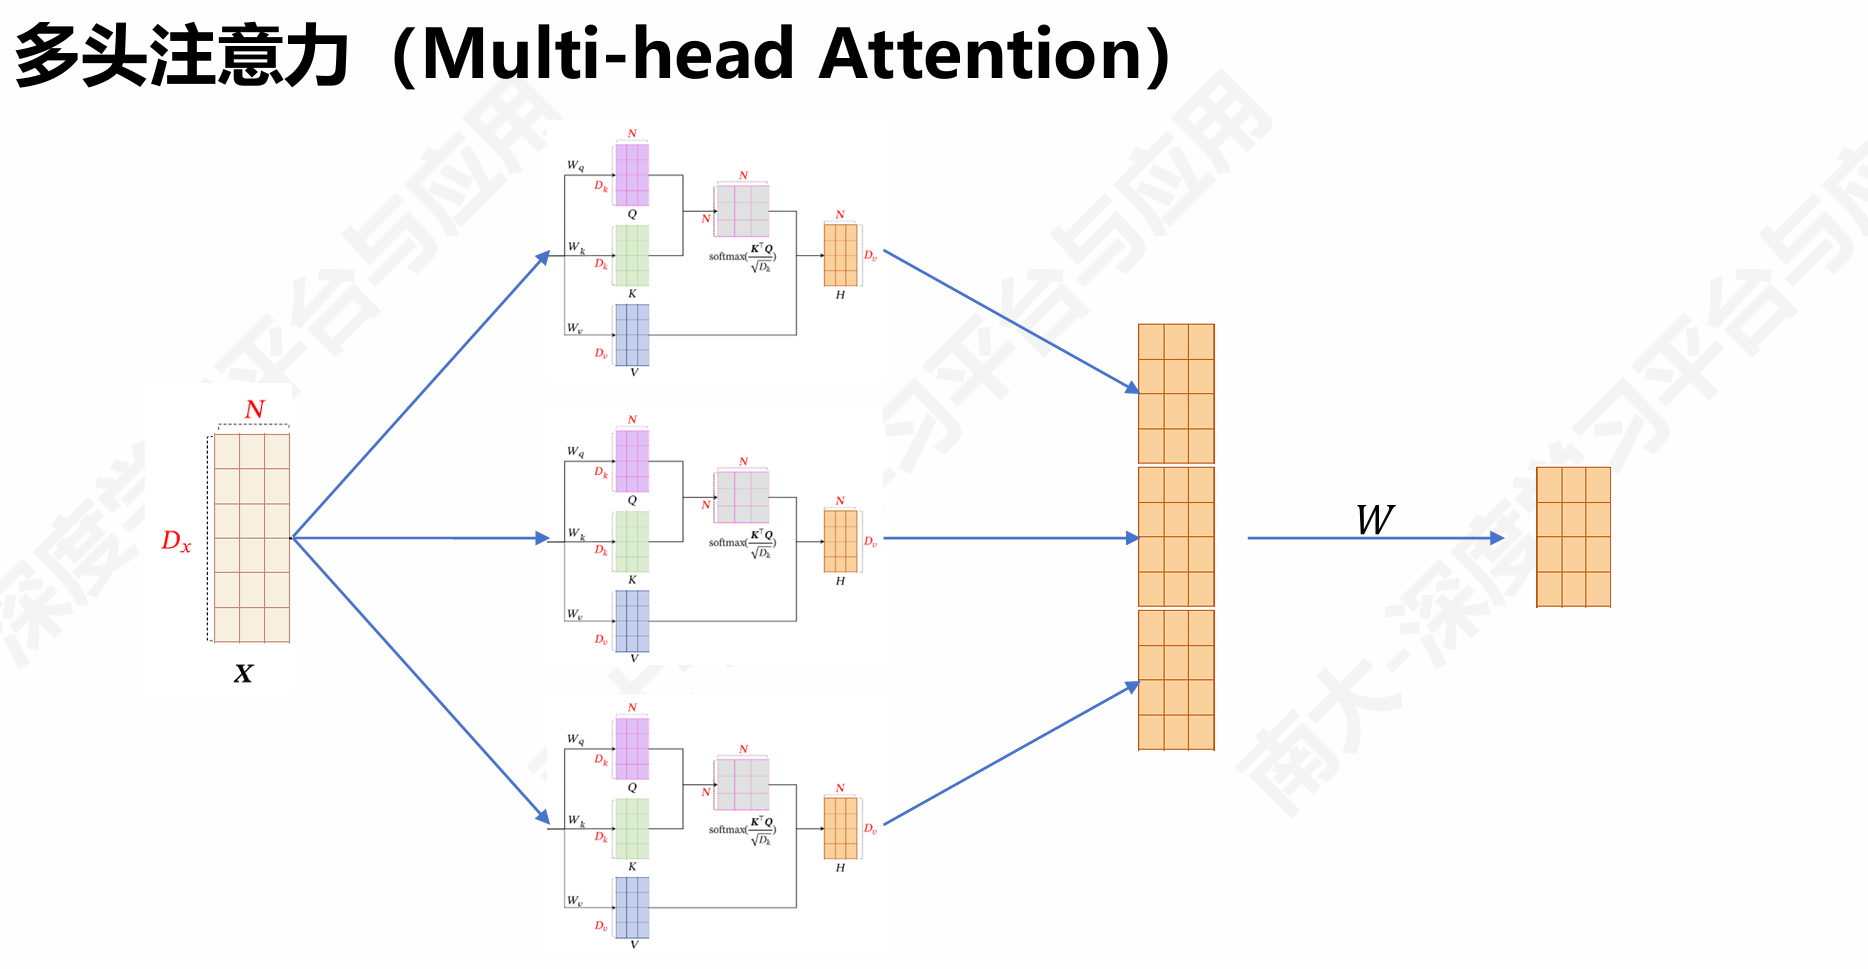
\includegraphics[width=0.5\linewidth]{Figures/5}
	\label{fig:5}
\end{figure}
		
		
		\vspace{10pt}
		
		\textbf{对比：}
		
		\textbf{单头注意力：}仅通过一个查询、键和值计算注意力，并返回加权和。其表达能力受限于一个线性变换的结果。
		
		\textbf{多头注意力：}通过多个头并行计算注意力，每个头独立地学习不同的表示子空间。最后将各个头的输出拼接，并进行线性变换，能够捕捉到更多的关系和模式。
	\end{sol}
	
	\newpage
	
	\begin{prob}
		\textbf{Transformer结构中encoder和decoder的区别有哪些?}
	\end{prob}
	
	\begin{sol}
	我认为区别主要在以下几个方面：\par
	\hs{0}\textbf{1. 功能:}
	\begin{itemize}
		\item \textbf{Encoder}：负责处理输入数据（如句子），将其转换为一个上下文相关的表示（即隐藏状态），这个表示被传递给Decoder。
		\item \textbf{Decoder}：生成输出数据（如翻译的句子），在生成过程中依赖于Encoder的输出和自身已经生成的部分。
	\end{itemize}
	
	\textbf{2. 输入和输出} 
	\begin{itemize}
		\item \textbf{Encoder}：输入是原始的序列数据，输出是对输入序列的深度表示（即隐层表示）。
		\item \textbf{Decoder}：输入包括Encoder的输出（编码后的表示）和Decoder自身已经生成的部分。Decoder的输出是一个概率分布，用于生成下一个单词或符号。
	\end{itemize}
	
	\textbf{3. 自注意力机制是否有遮蔽} 
	\begin{itemize}
		\item \textbf{Encoder}：每个Encoder层内有一个自注意力层，它通过关注输入序列的所有位置，计算每个位置对其他位置的依赖关系。自注意力机制没有遮蔽。
		\item \textbf{Decoder}：Decoder也有自注意力层，但与Encoder不同，Decoder的自注意力机制是\textbf{有遮蔽的}（Masked），即每个位置只能看到它自己以及之前的输出，以防止模型在生成时"偷看"未来的信息。
	\end{itemize}
	
	\textbf{4. 是否有Encoder-Decoder注意力机制} 
	\begin{itemize}
		\item \textbf{Encoder}：没有这个机制。Encoder只关注输入序列。
		\item \textbf{Decoder}：Decoder的每一层都有一个Encoder-Decoder注意力层，它允许Decoder在生成过程中，利用Encoder输出的上下文信息来调整生成的内容。
	\end{itemize}
	
	\textbf{5. 层数和复杂度} 
	\begin{itemize}
		\item \textbf{Encoder}和\textbf{Decoder}的结构基本相同，通常由多层（如6层）的Encoder和Decoder堆叠而成，每一层都包含自注意力机制、前馈神经网络以及在Decoder中的Encoder-Decoder注意力机制层。Decoder通常会比Encoder多一个额外的注意力机制层。
	\end{itemize}
		
	\end{sol}
	
	\newpage
	
	\section{目标检测（R-CNN）}
	
	\begin{prob}
		\textbf{请简要描述R-CNN模型的工作流程。具体来说，R-CNN是如何进行目标检测的？简述R-CNN模型的主要步骤。}
	\end{prob}
		
	\begin{sol}
		这个几个问题实际上都是问的一个问题，即R-CNN的工作步骤流程，流程如下：
		
		\begin{enumerate}
			\item \textbf{区域提议生成}：R-CNN首先使用一个选择性搜索（Selective Search）算法从输入图像中用\textbf{区域生成网络}生成多个候选区域（Regions of Interest（ROI））。这些区域可能包含目标物体或背景。
			选择性搜索通过多种策略（如颜色、纹理、大小和形状等）将图像分割成若干小区域，然后将这些区域逐渐合并，生成不同大小的候选区域。
			
			\item \textbf{特征提取：}每个图像区域使用\textbf{卷积网络处理 ImageNet 预训练的 CNN}。通常，使用的是像AlexNet这样的深度卷积神经网络，CNN会为每个候选区域提取一个固定长度的特征向量（通常是一个高维向量）。这些特征向量能很好地表示区域内部的视觉信息。
			
			\item \textbf{分类与回归：}对于每个候选区域的特征向量，R-CNN使用支持向量机（SVM）进行分类，判断该区域是否包含某个特定目标类别（例如人、车、猫等）。这个过程对于每个类别都需要\textbf{训练一个独立的SVM}。
			同时，R-CNN还会进行边界框回归（Bounding Box Regression），即预测该候选区域的准确边界框位置，通过微调候选区域的位置和大小，使其更精确地覆盖物体。即\textbf{对每个 RoI 预测调整值。}
			
			\item \textbf{最终检测结果输出:}对于所有候选区域，R-CNN会得到类别预测和边界框回归结果。然后，使用非极大值抑制（Non-Maximum Suppression, NMS）来去除重复的检测框，保留最准确的目标检测结果。
		
		\end{enumerate}
	\end{sol}
	
	\begin{prob}
		\textbf{与传统的R-CNN相比，Fast R-CNN的最大改进是什么？请简要说明Fast R-CNN如何避免了R-CNN中存在的冗余计算问题。}\
	\end{prob}
	
	\begin{sol}
	\textbf{最大改进：}\\
	传统R-CNN使用SVM对每个ROI分类的时候，有些区域会重复计算多次（被多个ROI覆盖的），从而产生``效率很低，非常慢"的问题。而Fast R-CNN的最大改进就是利用idea：``使用卷积网络处理整张图像，在特征上进行区域提取"，大大减少了重复计算，从而大大提高了处理速度。数值上，Fast R-CNN训练非常深的VGG16网络比R-CNN快9倍，在测试时快213倍。
	
	\textbf{具体如何避免了冗余计算：}
	\begin{enumerate}
		\item \textbf{使用卷积网络处理整张图像：}传统R-CNN一张图像内候选框之间大量重叠，提取特征操作冗余。而Fast R-CNN整个图像只需要通过一次卷积神经网络（CNN）。Fast R-CNN直接对整个图像计算卷积特征，然后通过区域提议（Region of Interest, RoI）将卷积特征映射到每个候选区域，大大减少了重复计算。
		\item \textbf{用ROI pooling层取代最后一层max pooling层： }Fast R-CNN 将分类和边界框回归任务统一为一个网络，在共享特征基础上完成。避免冗余计算的核心机制是Fast R-CNN 引入了 RoI 池化层（Region of Interest Pooling Layer），其关键在于：
		首先对整个输入图像执行一次 CNN 前向传播，生成共享的卷积特征图。
		对每个候选区域，通过 RoI 池化层将该区域在特征图上的对应部分提取出来，转化为固定大小的特征。这些固定大小的特征被用于后续的分类和边界框回归任务。
	\end{enumerate}
		
	除了避免冗余计算之外，Fast R-CNN 效率的提高还一部分在于实现了端到端的训练：Fast R-CNN网络末尾采用并行的不同的全连接层，可同时输出分类结果和窗口回归结果，实现了end-to-end的多任务训练，也不需要额外的特征存储空间。
	\end{sol}

\end{document}
